\documentclass[conference]{IEEEtran}
\usepackage{graphicx}
\usepackage{booktabs}
\usepackage{amsmath}
\usepackage{url}
\usepackage[hidelinks]{hyperref}
\renewcommand{\ttdefault}{cmtt}

\title{MediaPipe and DINOv2 Representations for Hand-Strength Prediction in Broadcast Poker}

\author{\IEEEauthorblockN{Minu Choi}
\IEEEauthorblockA{School of Data Science\\
University of Virginia\\
Charlottesville, VA\\
qce2dp@virginia.edu}}

\begin{document}
\maketitle

\begin{abstract}
Televised poker commentary and a recent broadcast ``AI bluff detector''
popularized the claim that nonverbal behavior reveals hand strength on
camera. We test that claim with a fully automated pipeline over 46.6 hours
of publicly broadcast cash-game footage with exposed hole cards: eight
sessions, 12{,}417 decisions, 9{,}801 of them with equity labels. Game
state is read from the broadcast graphics by OCR, hands are reassembled
into decision windows, and hand strength is labeled by Monte Carlo equity.
MediaPipe face and body streams are summarized into behavioral features
for camera-covered decisions of tracked players. Our central
methodological finding is an identity-contamination artifact. Under
progressively stricter face-attribution hygiene, an apparent behavioral
effect first strengthened to a nominally resolvable $\Delta$AUC of
$+0.096$ (95\% CI $[+0.005, +0.181]$), then vanished entirely ($+0.009$,
$[-0.058, +0.074]$) once every enrolled reference face was verified. The
spurious effect was produced by frames in which a lookalike neighbor was
silently credited to the tracked player. A preregistered replication on
two additional sessions, with the analysis frozen before download,
decisively failed: pooled across four sessions, face and pose features
change out-of-session AUC by $-0.075$ (95\% CI $[-0.134, -0.020]$,
$n=292$ covered decisions), with approximately 91\% power to detect the
registered $+0.096$. Sensitivity analyses show the degradation is not
estimator variance. No regularization scheme rescues the features; a
behavior-only model is anti-predictive out of session (AUC $0.349$, below
chance under a hand-level permutation test, $p = 0.018$); the effect
persists within a single player across his four sessions. A second
preregistered round resolved the within-session question on all eight
sessions: behavior-only AUC is $0.587$ (95\% CI $[0.515, 0.655]$,
$n=494$), excluding chance under the frozen criterion, while
cross-session transfer stays at or below chance ($0.430$,
$[0.358, 0.502]$). A preregistered frozen DINOv2 probe adds nothing over
betting action out of session ($+0.012$, $[-0.079, +0.103]$), extending
the conclusion to learned representations. Tells exist and are
machine-readable within a session, and they do not transfer across
sessions. Decision timing, which needs no camera, is bounded below
$+0.01$ AUC over betting action. We conclude that identity hygiene, not
feature engineering, is the binding methodological risk for behavioral
video datasets built on multi-person footage, and that behavioral
hand-strength models of this class do not generalize across sessions.
\end{abstract}

\begin{IEEEkeywords}
nonverbal behavior, poker, deception detection, person re-identification,
preregistration, broadcast video analysis, negative results
\end{IEEEkeywords}

\section{Introduction}

Poker folklore holds that players leak the strength of their hands through
nonverbal ``tells,'' and the 2026 World Series of Poker broadcast
popularized the idea that such leakage is machine-readable, overlaying a
behavioral hand-strength model on live coverage. The scientific evidence
behind that idea is thinner than its television presence suggests. The best
controlled result reports that naive observers judge professional players'
hand quality above chance from arm movements alone, at modest effect sizes,
while judgments from the face are at or below chance
\cite{slepian2013quality}. Automated deception detection benchmarks report
within-domain accuracies in the sixties and cross-domain transfer barely
above chance \cite{guo2023dolos}. No prior work, to our knowledge, has
tested the broadcast-poker claim end to end: does adding automatically
extracted nonverbal behavior improve prediction of hand strength over the
betting action alone, evaluated out of session, on public footage?

This paper contributes four things.

\textbf{(1) A reproducible pipeline} that converts raw broadcast video into
a labeled decision-level dataset. The stages are OCR of the broadcast
graphics package into per-second game-state snapshots, a state machine
that reassembles hands and decision windows, Monte Carlo equity labels
from the exposed hole cards, and per-decision behavioral features from
face landmarks, blendshapes, and body pose. Features carry per-player
normalization and explicit bet-size leakage controls. A released demo
renderer overlays every extracted signal on the source broadcast
(Figure \ref{fig:demo}).

\textbf{(2) An identity-contamination case study} (Section
\ref{sec:artifact}). Behavioral datasets built on multi-person footage must
attribute every measured face to the right person. We document three small
engineering gaps: an open-set similarity threshold, nondeterministic
reference enrollment, and unbounded nearest-position matching. Together
they let a lookalike neighbor's face be silently measured as the tracked
player's. The resulting artifact produced an apparently resolvable
behavioral effect that grew under partial cleaning and vanished under full
cleaning (Figure \ref{fig:arc}). We distill the fix into a verification
protocol.

\textbf{(3) A preregistered, adequately powered replication failure}
(Section \ref{sec:prereg}). With the analysis frozen before the new footage
was downloaded, face and pose features reduce pooled out-of-session AUC by
$0.075$ (95\% CI $[-0.134, -0.020]$). The study had approximately 91\%
power to detect the registered positive estimate.

\textbf{(4) A session-locality finding} (Section \ref{sec:sensitivity}).
Behavioral features are not merely uninformative out of session: a
behavior-only model scores AUC $0.349$, significantly below chance under
a hand-level permutation test ($p = 0.018$), and the inversion persists
within the same player across his four sessions. Within sessions the same
features carry real signal, resolved in a second preregistered round on
eight sessions (pooled $0.587$, CI $[0.515, 0.655]$, excluding chance).
Learned behavior-to-strength associations are session-specific in sign:
real enough to fit, wrong enough to mislead on a new night. Tells are
session-local, at both ends of the claim.

\begin{figure*}[t]
\centering
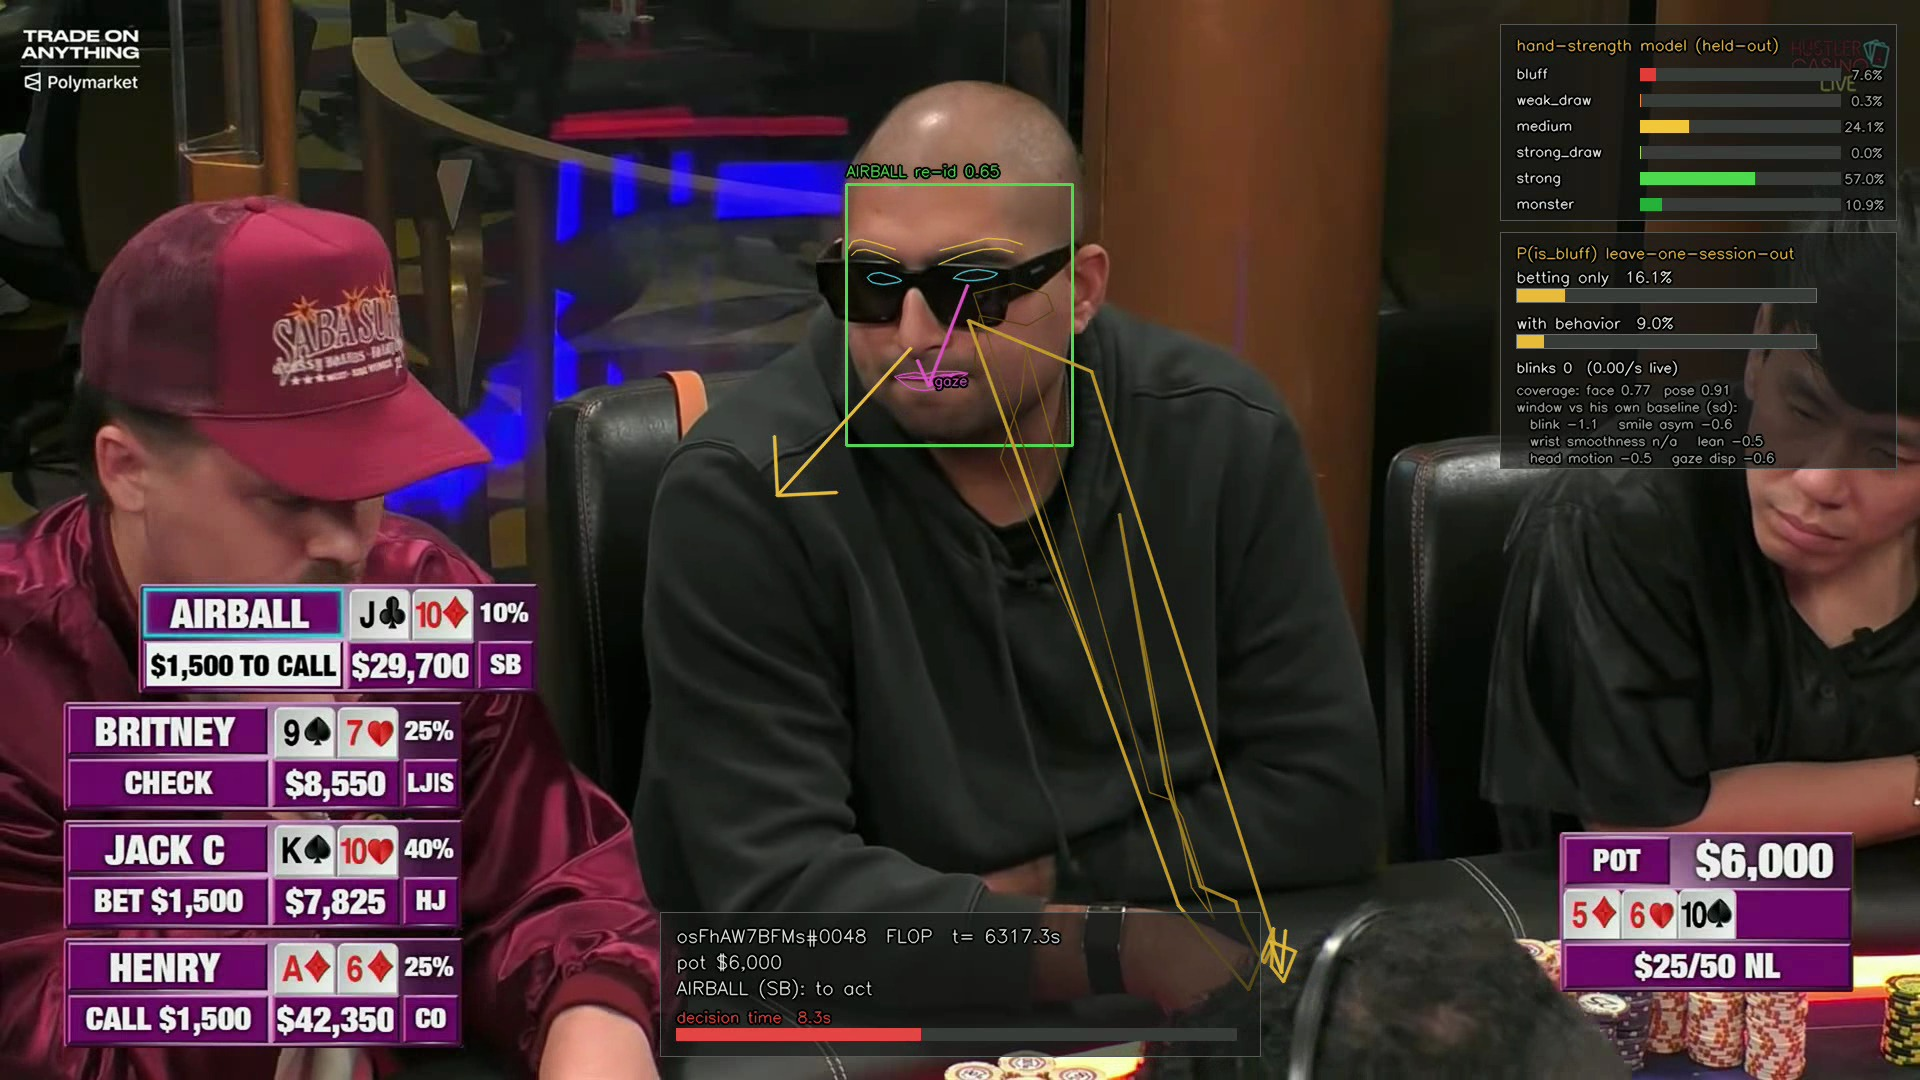
\includegraphics[width=\textwidth]{figures/demo_frame.jpg}
\caption{One annotated frame from the released demo renderer (July 2026
(b) session, hand 48, flop decision). Green box: identity-gated face
attribution with its re-identification score. Colored contours are
MediaPipe face landmarks (brows, eyes, lips); the magenta ray is the
gaze vector, the yellow arrow the head direction, and the yellow trace
the One-Euro-filtered acting-wrist path that feeds the kinematic
features. Top right: the held-out six-class strength distribution, the
\texttt{is\_bluff} probability with and without behavioral features,
and live per-window readouts standardized against the player's own
baseline. Bottom center: hand identifier, street, pot, actor, and
decision clock from the OCR game state. The purple player panels and
pot graphics are part of the source broadcast.}
\label{fig:demo}
\end{figure*}

\section{Related Work}

\textbf{Poker AI plays cards, not people.} Superhuman poker agents
reached and then surpassed top human play from game state and betting
action alone \cite{brown2018superhuman}, \cite{brown2019superhuman}. No
behavioral channel appears anywhere in that line of work. Whether human
nonverbal behavior carries residual, machine-readable signal on top of
the betting action is exactly the claim the broadcast overlay
popularized, and the one we test.

\textbf{Behavioral cues to poker hand strength.}
Slepian et al.\ \cite{slepian2013quality} showed observers rate hand quality above chance
from short clips of arm motion (smoothness of the chip push), while
face-only clips were directionally below chance. This motivates our
smoothness features and our expectation that any true effect is small. Work
on automated deception detection in the wild reports within-domain
accuracy around 60 to 67 percent on gameshow and courtroom corpora and
severe degradation across domains \cite{guo2023dolos}. Cross-session
failure of this kind is dataset shift \cite{quinonero2009dataset}: the
deployment distribution differs from training in ways the model cannot
see. Our result extends this pattern to a naturalistic, high-stakes,
repeated-game setting with objective ground truth, and sharpens it to
shift across nights within one venue, one broadcast package, and one
player.

\textbf{Person identification hygiene.} Face verification
\cite{deng2019arcface} and person re-identification \cite{zheng2016person}
under compression, occlusion, and pose variation are well studied;
sunglasses are endemic at poker tables. Deciding whether a detected face
belongs to an enrolled identity at all is the classic open-set problem
\cite{scheirer2013open}, and our initial fixed-threshold gate is exactly
the naive open-set design that literature warns against. What is
underappreciated is the role of attribution error as a silent noise
channel in downstream behavioral datasets. Label errors are known to
destabilize benchmark conclusions \cite{northcutt2021pervasive}; our
artifact is the feature-side analogue, attribution noise manufacturing a
positive finding out of another person's face.

\textbf{Methodological safeguards.} We use preregistration
\cite{nosek2018preregistration}, grouped bootstrap confidence intervals
\cite{efron1993bootstrap}, and leakage review of engineered features.
Trajectory smoothness metrics follow \cite{balasubramanian2015analysis}, \cite{hogan2009sensitivity}; keypoint trajectories are One-Euro
filtered \cite{casiez2012one} before any derivative is taken; face and
pose streams come from MediaPipe \cite{lugaresi2019mediapipe}; OCR uses
PP-OCR \cite{du2020ppocr}.

\section{Data}
\label{sec:pipeline}

\textbf{Footage.} Eight complete Hustler Casino Live cash-game sessions
(October 2025 to July 2026, 46.6 hours total) featuring one high-volume
professional (all eight sessions) and a second recreational player (one
session). Round 1 used four of them: the February, April, and both July
(a) and (b) broadcasts of 2026. The October, December, March, and July
(c) sessions were added under the round 2 preregistration. The stream
exposes hole cards in its graphics, providing ground truth without any
inference from behavior.

\section{Methodology}

\subsection{Preprocessing and Game-State Extraction}
Region-cropped OCR reads the pot, stakes, board, and
per-player panels (name, stack, action text, amount to call) once per
second. Card sprites are template-matched with a saturation-gated
segmentation robust to the two background styles in our footage. A state
machine folds snapshots into hands and decision windows: a window opens
when a player's panel shows an amount to call and closes at their action
flip. Cutaway gaps are re-merged when positions and hole cards agree, and
a preroll filter drops inset replays of older sessions. Table
\ref{tab:data} summarizes the result: 1{,}461 hands and 12{,}417
decisions across the eight sessions, 9{,}801 of them with equity labels.
Labels are Monte Carlo equity versus a random hand with deterministic
seeds, binned into six strength classes; \texttt{is\_weak} marks
decisions taken with equity below 0.45, and \texttt{is\_bluff} marks
aggressive such decisions.

\subsection{Behavioral Feature Extraction}
For each decision window of a mapped player, frames are searched for the
player's face (Section \ref{sec:artifact}). Accepted frames contribute
blendshape series: blink rate, smile asymmetry and mean, gaze dispersion,
and brow activity. A pose crop that follows the accepted face contributes
posture and wrist kinematics: lean variability, head motion, normalized
wrist peak speed, spectral arc length, and negative log dimensionless
jerk, which is amplitude-invariant by construction and therefore cannot
encode bet size. Six event detectors (downward-gaze rate, hand near face,
freeze fraction and longest freeze, chip-shuffle periodicity, forward
lean) are rates, fractions, ratios, or shoulder-width geometry, and
passed the same leakage review. Earlier two-session analyses showed the
detectors carry no signal, so the preregistration excluded them from the
primary test; Section \ref{sec:sensitivity} confirms the null on the
pooled data. All features are z-scored per player. Coverage is honest and
low: the primary player's face passes identity gating in 10 to 33 percent
of window frames depending on session. In the round 1 sessions, 292
labeled decisions meet the 0.5 coverage threshold; across all eight
sessions, 494 do.

\subsection{Evaluation Protocol}
Leave-one-session-out (LOSO): models train on all
other sessions and predict the held-out session; predictions are pooled.
Baselines use betting features only (position, sizing ratios, pot odds,
street, prior raises, stack-to-pot, timing). Deltas are reported with
hand-grouped bootstrap 95\% CIs (2{,}000 resamples), resampling hands so
correlated decisions within a hand never narrow the interval.


\begin{table}[t]
\centering
\footnotesize
\setlength{\tabcolsep}{3.5pt}
\caption{Dataset summary. A decision is covered when at least half of its
window frames pass identity gating (face) or pose tracking for a mapped
player; only covered, labeled decisions enter the ablations. Round 1
comprises Feb, Apr, Jul (a), and Jul (b) 2026; the other four sessions
were added in round 2.}
\label{tab:data}
\begin{tabular}{lrrrrrr}
\toprule
Session & Hours & Snapshots & Hands & Decisions & Labeled & Covered \\
\midrule
Oct 2025     & 6.7 & 22{,}636 & 156 & 1{,}736 & 1{,}079 & 75 \\
Dec 2025     & 6.4 & 22{,}774 & 196 & 1{,}814 & 1{,}223 & 26 \\
Feb 2026     & 5.2 & 17{,}501 & 141 & 1{,}320 & 1{,}163 & 114 \\
Mar 2026     & 6.4 & 21{,}851 & 212 & 1{,}770 & 1{,}511 & 31 \\
Apr 2026     & 5.5 & 18{,}814 & 164 & 1{,}188 & 1{,}027 & 55 \\
Jul 2026 (a) & 5.2 & 18{,}436 & 225 & 1{,}561 & 1{,}278 & 51 \\
Jul 2026 (b) & 5.9 & 20{,}730 & 192 & 1{,}570 & 1{,}347 & 72 \\
Jul 2026 (c) & 5.3 & 18{,}011 & 175 & 1{,}458 & 1{,}173 & 70 \\
\midrule
Total        & 46.6 & 160{,}753 & 1{,}461 & 12{,}417 & 9{,}801 & 494 \\
\bottomrule
\end{tabular}
\end{table}

\subsection{Identity Attribution}
\label{sec:identity}

Attributing faces on a multi-person broadcast requires deciding, per
frame, whether a detected face is the tracked player. Our initial design
used an open-set rule: accept the first face whose equalized grayscale
patch correlates at least $0.55$ with any enrolled reference patch of the
player, a threshold chosen from a measured same-player/cross-player
separation of $0.74$ versus $0.25$. Section \ref{sec:artifact} documents
how three gaps in this design manufactured a spurious finding; the
corrected protocol is: (i) enroll references deterministically, one
detector instance per reference frame; (ii) bound enrollment by position
and refuse specifications whose intended face is not found; (iii) verify
every enrolled patch by eye; (iv) sweep each session for faces that score
above threshold against the references, and register every non-target
such face as a distractor; (v) attribute a face only if it clears the
threshold and beats every distractor score by a margin, best candidate
wins; (vi) treat staff and commentators as candidate distractors too (one
of ours scored $0.60$).

\section{Models}
\label{sec:models}

Every model in the pipeline was chosen under three constraints. The
corpus is large in hours but small in supervised examples: hundreds of
camera-covered decisions, not tens of thousands. The footage is
compressed 1080p broadcast video, so perception components must tolerate
compression, cutaways, and occlusion. And the study's claims rest on
auditability, so each stage must produce outputs a human can verify.

\textbf{Game-state reading.} Broadcast graphics are read by the PP-OCRv6
detection and recognition models (tiny tier) of the PP-OCR family
\cite{du2020ppocr}, applied to fixed regions so the recognizer sees one
panel at a time. The graphics package is a fixed template, so the
problem is throughput rather than layout understanding: per-second
sampling of 46.6 hours yields 160{,}753 snapshots, all processed on CPU.
Card sprites are identified by normalized template correlation instead
of a learned detector because the sprite set is closed and rendered
deterministically, which makes template matching both exact and
inspectable.

\textbf{Behavioral streams.} Face geometry, blendshapes, and body
keypoints come from the MediaPipe Face Landmarker and Pose Landmarker
(lite) models \cite{lugaresi2019mediapipe}. We chose MediaPipe because
its blendshape outputs are named, interpretable facial signals (blink,
smile, brow, gaze) that map directly onto the tells discussed in the
poker literature, and because both landmarkers run at broadcast frame
rates on CPU, which the 46.6-hour corpus requires.

\textbf{Identity matching.} Faces are attributed by correlation of
equalized grayscale patches against enrolled references rather than by a
deep face embedding such as ArcFace \cite{deng2019arcface}. The choice
is deliberate: every acceptance is a comparison against a reference
patch a human has verified, and the artifact study of Section
\ref{sec:artifact} depends on being able to inspect exactly what the
matcher saw. A stronger embedding would widen the match margin but faces
the same open-set decisions that Section \ref{sec:identity} addresses by
protocol.

\textbf{Hand-strength labels.} Equity is computed by Monte Carlo
simulation against a random opponent hand using the \texttt{treys}
evaluator with deterministic seeds. Equity versus a random hand ignores
opponents' actual ranges; we accept that simplification because it
requires no modeling assumptions and is computed identically across
sessions, so it cannot introduce session-specific label bias.

\textbf{Analysis models.} All primary tests use logistic regression
(scikit-learn \cite{pedregosa2011scikit}, $C=1.0$) on standardized,
median-imputed features, and ridge regression for the continuous-equity
arm. A linear probe is the standard instrument for asking whether a
representation carries signal, and with $n=292$ to $494$ covered
decisions, anything more flexible would mostly measure its own variance.
Stronger and sparser regularization variants (L2 at $C=0.1$ and $0.01$,
L1 at $C=0.1$ and $0.05$) are reported as sensitivity arms in Section
\ref{sec:sensitivity}.

\textbf{Learned representation.} Round 2 tests whether hand-crafted
summaries are the bottleneck by replacing them with DINOv2 ViT-S/14
embeddings \cite{oquab2024dinov2}, kept frozen. Identity-gated face
crops and their pose crops are embedded per frame, pooled to the
per-window mean and standard deviation, and reduced by PCA to 32
components fit on training folds only. DINOv2 was chosen as a strong
general-purpose self-supervised representation that transfers without
fine-tuning; freezing it keeps the probe protocol identical to the
hand-crafted arm and avoids fitting tens of millions of parameters to
hundreds of examples.

\section{Results}

\subsection{The Identity-Contamination Artifact}
\label{sec:artifact}

\begin{figure}[t]
\centering
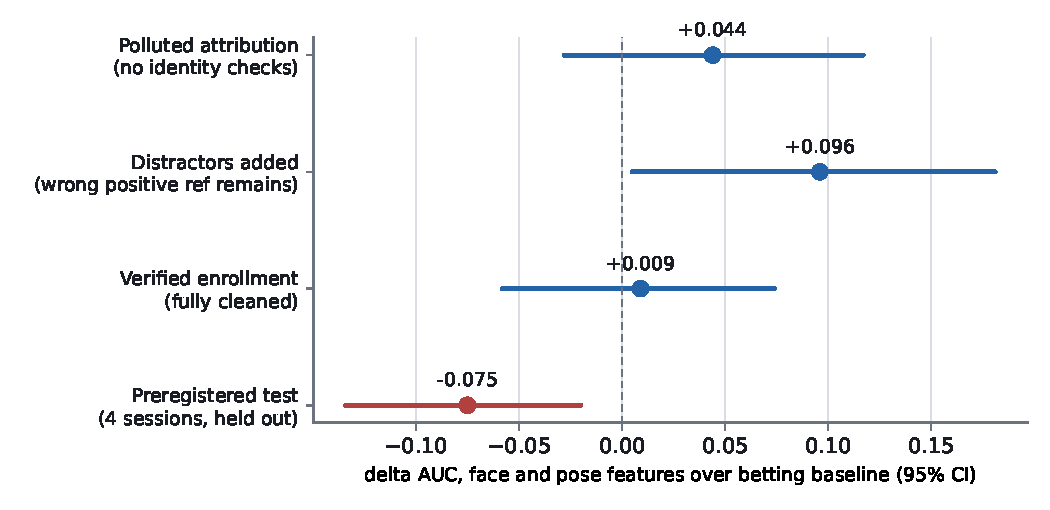
\includegraphics[width=\linewidth]{figures/artifact_arc.pdf}
\caption{An apparent behavioral effect tracks attribution pollution, not
behavior. Points are $\Delta$AUC of face and pose features over the
betting baseline for \texttt{is\_weak} with hand-grouped bootstrap 95\%
CIs. The first three estimates are in-sample over two sessions under
progressively stricter identity hygiene; the fourth is the preregistered
four-session test.}
\label{fig:arc}
\end{figure}

Three gaps in the initial identity design of Section
\ref{sec:identity} turned face attribution into a contamination channel.

\textbf{Gap 1: lookalikes above threshold.} A neighboring player
correlated $0.66$ with the tracked player's references. Whenever the
tracked player's face dipped out of detectability (chin on hand, looking
down), the neighbor was accepted in his place. In one session, 82 of 193
windows contained some wrong-person frames; one window was entirely the
neighbor.

\textbf{Gap 2: nondeterministic enrollment.} Reference patches were
enrolled by seeking to hand-verified timestamps and taking the detected
face nearest a specified position. Detection under a warm video-mode
tracker is stateful: which faces are found at a seek depends on the seeks
before it. Re-runs enrolled different faces from the same specification.

\textbf{Gap 3: unbounded nearest-position matching.} When the intended
player went undetected at a reference timestamp, the nearest detected face
was enrolled with no distance bound. In two of four sessions this placed a
neighbor's face inside the player's positive reference library, which also
neutralized the distractor defense added after Gap 1: the enrolled
lookalike outscored his own distractor reference.

Figure \ref{fig:arc} shows the consequence. With no identity checks the
apparent effect was $+0.044$ $[-0.028, +0.117]$. After registering the
known lookalike as a distractor, but with a wrong face still enrolled as a
positive reference, the effect strengthened to $+0.096$ $[+0.005, +0.181]$,
nominally resolvable. With enrollment made deterministic (fresh tracker
per reference frame), position-bounded (a face must lie within 110 px of
its specification), and every enrolled patch visually verified, the
in-sample effect collapsed to $+0.009$ $[-0.058, +0.074]$. The mechanism
is mundane: another person's face, measured during the tracked player's
decisions, covaries with decision context (cameras cut to neighbors during
long tanks) in ways that imitate a tell.

\subsection{Preregistered Replication}
\label{sec:prereg}

Before downloading any new footage we froze, in a committed
preregistration document: the hypothesis (face and pose features improve
pooled LOSO AUC for \texttt{is\_weak}), the registered estimate
($+0.096$), the exact pipeline settings, the seat-mapping discipline for
new sessions (commit-moment identification and a distractor audit before
any model output), the pass criterion (pooled CI excluding zero on the
positive side), and a prohibition on post-hoc adjustment. Two sessions
were selected by roster and layout compatibility; one candidate was
excluded before extraction because it used a different graphics package,
and the exclusion was logged in the preregistration.

The pooled four-session test returned
\[
\Delta\mathrm{AUC} = -0.075,\quad 95\%\ \mathrm{CI}\ [-0.134,\ -0.020],
\quad n = 292.
\]
The CI excludes zero on the negative side: added behavioral features
reduce out-of-session performance. Under a normal approximation to the
bootstrap distribution (SE $\approx 0.029$), the test had approximately
91\% power to detect the registered $+0.096$, and 80\% power for any
delta of at least $+0.082$. The upper confidence bound rules out all
positive effects at the 2.5\% level. The betting-only baseline itself
scores AUC $0.549$ pooled out of session, against $0.75$ within session,
replicating the known brutality of cross-session transfer.

\subsection{Model Results: Why Negative, Not Just Null}
\label{sec:sensitivity}

\begin{figure}[t]
\centering
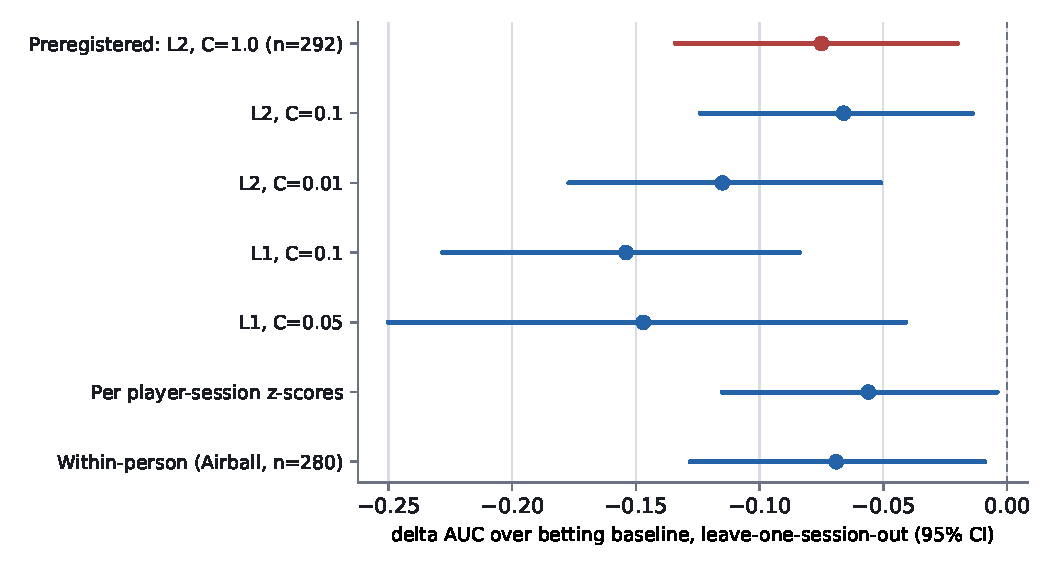
\includegraphics[width=\linewidth]{figures/sensitivity_forest.pdf}
\caption{No analysis choice rescues the features (round 1: pooled LOSO
over the four round 1 sessions). All arms are $\Delta$AUC over the
betting baseline for \texttt{is\_weak} with hand-grouped bootstrap 95\%
CIs.}
\label{fig:forest}
\end{figure}

A significantly negative delta invites the objection that the estimator,
not the signal, is at fault: ten added dimensions can hurt a small model
even when they carry information. Four analyses reject this reading
(Figure \ref{fig:forest}).

\textbf{Regularization does not help.} Stronger L2 shrinkage leaves the
delta unchanged or worse ($C=0.01$: $-0.115$), and sparse L1 selection is
worst of all ($-0.154$): selecting the few behavioral features that look
best in training amplifies reliance on associations that do not hold in
the held-out session.

\textbf{Behavior alone is anti-predictive.} A behavior-only model scores
AUC $0.349$, far below chance. Whatever association the model learns
between behavior and weakness in three sessions, the reverse tends to hold
in the fourth. Under label exchange this would be signal; under session
exchange it is instability.

\textbf{The inversion survives within a person.} Restricted to the primary
player's four sessions (one identity, one seat style, $n=280$), the delta
is $-0.069$ $[-0.128, -0.009]$. Idiosyncrasy across people does not
explain the failure; instability within a person across nights does.

\textbf{Session geometry explains only part.} Re-standardizing features
per player-session (removing session-level offsets induced by camera
geometry, since a lean angle or apparent motion scale depends on the shot)
moves the behavior-only AUC from $0.349$ to $0.387$ and the delta to
$-0.056$ $[-0.115, -0.004]$. Session offsets are therefore a real
confound channel that future work must normalize away, and still not the
whole story.


\begin{figure}[t]
\centering
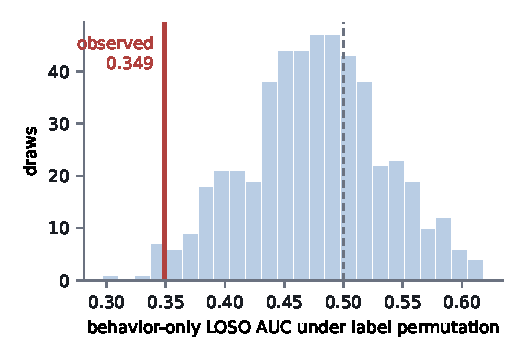
\includegraphics[width=\columnwidth]{figures/permutation_null.pdf}
\caption{The below-chance transfer is significant (round 1). Hand-level
label permutations within each session, re-running the full
cross-session pipeline per draw (500 draws), place the observed
behavior-only AUC in the null's lower tail ($p = 0.018$).}
\label{fig:perm}
\end{figure}

\begin{figure}[t]
\centering
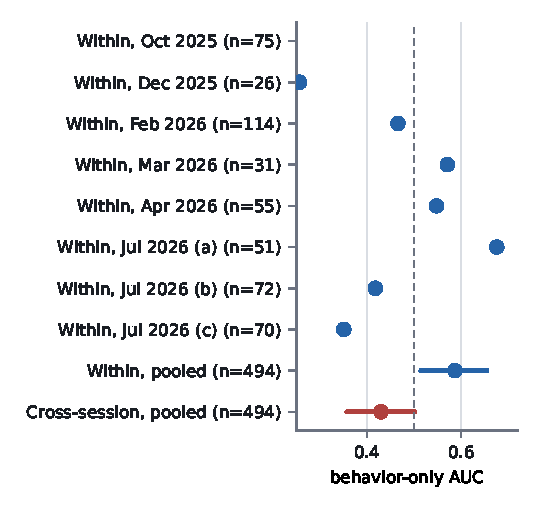
\includegraphics[width=\columnwidth]{figures/session_locality.pdf}
\caption{Session locality, resolved on eight sessions (round 2).
Within-session grouped cross-validation finds real but heterogeneous
behavioral signal (pooled CI excludes chance); the same features
transfer at or below chance across sessions.}
\label{fig:locality}
\end{figure}

\textbf{The inversion is significant; within-session signal was marginal
in round 1.} Two further analyses locate the failure precisely. First, a
permutation test that shuffles labels at the hand level within each
session and re-runs the full cross-session pipeline places the observed
behavior-only AUC of $0.349$ (hand-grouped bootstrap CI $[0.279, 0.429]$,
entirely below chance) in the lower tail of its null (null mean $0.476$,
SD $0.058$, $p = 0.018$; Figure \ref{fig:perm}): transfer is not merely
absent but systematically inverted. Second, within-session grouped
cross-validation (5-fold by hand, per session, pooled over the four
round 1 sessions) gives a behavior-only AUC of $0.574$ with a
hand-grouped bootstrap CI of $[0.492, 0.652]$ and per-session values
from $0.418$ to $0.676$; Section \ref{sec:round2} resolves this estimate
on all eight sessions (Figure \ref{fig:locality}). Together these say
the model is not hallucinating. It finds real within-session structure
in at least some sessions, but the sign of that structure is
session-specific (Table \ref{tab:signs}: no feature keeps its fitted
sign across all four round 1 sessions), so exporting it is worse than
ignoring behavior. This is the paper's clearest positive
characterization: behavioral hand-strength associations in this setting
are session-local.

\textbf{The event detectors are a true null, not an inversion.} As
secondary arms on the pooled four-session data, the six leakage-proofed
event detectors alone give $+0.011$ $[-0.037, +0.063]$, and the union of
all behavioral features gives $-0.060$ $[-0.128, +0.005]$. The contrast
with face and pose is instructive: the low-dimensional detectors, built
as rates and ratios with explicit leakage review, neither help nor hurt,
while the richer face and pose summaries are the source of the inversion.

\subsection{Decision Timing and Continuous Targets}

Two further analyses use the label information more efficiently.
\textbf{Decision timing at full power.} Time to act needs no camera, so
it is available for all 4{,}815 labeled decisions of every player in the
round 1 sessions, not just the 292 camera-covered ones. Added to the
betting baseline it changes \texttt{is\_weak} AUC by $+0.004$ (95\% CI
$[-0.002, +0.010]$) and \texttt{is\_bluff} by $-0.000$
$[-0.005, +0.004]$: the most cited poker tell, tank duration, is bounded
below one hundredth of AUC in this setting. \textbf{Continuous equity.}
Regressing Monte Carlo equity directly (ridge, out-of-session Spearman
correlation) uses the full label rather than a threshold. The face and
pose degradation replicates and tightens ($\Delta\rho = -0.099$, CI
$[-0.144, -0.047]$ on covered rows), while timing shows the study's only
resolvable positive effect, at negligible magnitude
($\Delta\rho = +0.005$, CI $[+0.002, +0.008]$, $n = 4{,}815$). The
latter matters mainly as a sensitivity check: the pipeline and
evaluation resolve genuinely small effects when the sample allows, so
the behavioral nulls are not an artifact of blunt instruments.

\begin{table}[t]
\centering
\footnotesize
\caption{No behavioral feature keeps its coefficient sign across all
four round 1 sessions (behavior-only logistic model per session,
\texttt{is\_weak}, standardized features; $+$/$-$ is the fitted sign).}
\label{tab:signs}
\begin{tabular}{lcccc}
\toprule
Feature & Feb & Apr & Jul (a) & Jul (b) \\
\midrule
blink rate & $+$ & $-$ & $+$ & $+$ \\
smile asymmetry & $-$ & $-$ & $-$ & $+$ \\
smile mean & $+$ & $-$ & $+$ & $-$ \\
gaze dispersion & $+$ & $-$ & $+$ & $+$ \\
brow activity & $+$ & $+$ & $+$ & $-$ \\
wrist peak speed & $+$ & $+$ & $-$ & $-$ \\
wrist smoothness (LDJ) & $+$ & $+$ & $-$ & $+$ \\
wrist SPARC & $+$ & $+$ & $-$ & $-$ \\
lean variability & $-$ & $-$ & $-$ & $+$ \\
head motion & $-$ & $-$ & $+$ & $-$ \\
\bottomrule
\end{tabular}
\end{table}

\subsection{Round 2: Preregistered Resolution and Learned Representations}
\label{sec:round2}

A second preregistration, committed before any round 2 footage was
downloaded, fixed two experiments: four additional sessions to resolve
the within-session estimate, and the frozen DINOv2 probe of Section
\ref{sec:models} to test whether a learned representation changes the
out-of-session answer.

\textbf{Within-session signal is real.} Pooled within-session grouped
cross-validation across all eight sessions gives a behavior-only AUC of
$0.587$ with a hand-grouped bootstrap 95\% CI of $[0.515, 0.655]$
($n=494$), excluding chance under the frozen resolution criterion
(Figure \ref{fig:locality}). Per-session values remain strongly
heterogeneous ($0.26$ to $0.76$). The best session ($0.756$) is the one
in which the primary player wore no sunglasses, though the second
bare-faced session scores low at small $n$, so the occlusion account
stays a hypothesis. The cross-session arm on the same enlarged pool
stays at or below chance (behavior-only $0.430$, CI $[0.358, 0.502]$;
face and pose delta over betting $-0.034$, CI $[-0.080, +0.012]$). The
session-locality claim is thereby resolved at both ends: tells exist
within a night and do not transfer across nights.

\textbf{A learned representation does not change the answer.} The
preregistered DINOv2 probe adds $+0.012$ over the betting baseline out
of session (CI $[-0.079, +0.103]$, $n=257$ embedding-covered
decisions): a null, extending the conclusion from hand-crafted features
to a standard frozen representation. Two nuances are worth recording.
The embedding probe alone transfers at $0.545$, above the inverted
hand-crafted features, so embeddings are uninformative rather than
misleading out of session. Within sessions the probe scores $0.398$
(CI $[0.320, 0.476]$), below chance where the ten hand-crafted features
find real signal. At these sample sizes, a 1536-dimensional
representation reduced to 32 components is less stable than ten
purpose-built features, a capacity lesson for small behavioral corpora.

\section{Discussion}

Three readings of these results deserve separation. The narrow reading is
engineering: with tabular summary features over MediaPipe streams, a
linear model, eight sessions, and camera-limited coverage,
out-of-session behavioral signal is not extractable, and the attempt
costs accuracy. The middle reading is statistical. Effects of the size
the literature supports, a few hundredths of AUC, require an order of
magnitude more covered decisions than 46.6 hours of broadcast yields.
Any study in this regime that reports a large positive behavioral effect
should therefore be audited first for identity contamination, which we
show can manufacture exactly such an effect. The broad reading is
substantive. Even within one professional, behavior-strength
associations invert across nights, which is what one expects if
experienced players' surface behavior is dominated by context, table
dynamics, and deliberate randomization rather than stable leakage.
Round 2 resolves the distinction that round 1 could not: tells exist
(within-session signal excludes chance under a preregistered criterion)
and are contextual and unstable across nights, which entails that
broadcast-scale models of this class cannot use them out of session.

The artifact deserves the emphasis we give it. It produced, in our own
hands, a preregistration-worthy positive estimate with a confidence
interval excluding zero, out of nothing but face misattribution. It grew
stronger under partial cleaning because the partially cleaned pipeline
retained the most correlated contamination. Behavioral-video findings
built on multi-person footage without an explicit attribution audit
should be treated as provisional.

\section{Limitations}

One primary player carries most covered decisions; sunglasses make eye
features noise for him, as for many poker subjects. Coverage is bound by
broadcast camera direction, not by us. Card-reading errors survive at a
low rate (rank confusions on small sprites) and add label noise to equity.
The betting baseline is deliberately simple; a stronger baseline would
only shrink headroom for behavior. Our features are window-level
summaries. Sequence models over raw streams remain untested here, though
they face the same coverage and identity constraints with more capacity
to overfit them. Two round 2 observations mark future work rather than
conclusions. The best within-session score came from the one session in
which the primary player wore no sunglasses, so occlusion may bound the
face channel; a targeted comparison of bare-faced versus occluded
sessions would test that directly. And the DINOv2 probe scored below
chance within sessions where ten purpose-built features found signal,
suggesting that representation capacity at this sample size, not
representation quality, is what binds; the remedy is more covered
decisions, not bigger models.

\section{Conclusion}

We built an end-to-end pipeline from broadcast poker video to labeled
decision-level behavioral data and asked whether nonverbal behavior adds
predictive power over betting action for hand strength. Under a
preregistered and adequately powered test, the answer is that it
subtracts out of session. Behavior-strength associations are learnable
within a session, but their signs are session-specific, so models that
carry them to a new session perform significantly below chance. Along
the way we showed how easily the opposite conclusion is manufactured: a
single misattributed face in a reference library produced a nominally
significant positive effect that survived partial cleaning. The
attribution-hygiene protocol, the preregistrations, and the full
analysis history are released with the code. For behavioral video
research, the order of operations this study recommends is: verify
identity first, preregister second, and only then believe an effect.

\section{Ethics and Reproducibility}

All footage is publicly broadcast with player consent to the stream's
hole-card exposure. We analyze it post hoc and redistribute no footage;
the single annotated frame in Figure \ref{fig:demo} is reproduced from
the public broadcast to illustrate the system. We publish code, derived
features, timestamps, and the preregistrations rather than clips. Pipeline, analysis code,
seat maps, audit tooling, figure scripts, and the frozen
preregistrations with their logged results are available at
\url{https://github.com/minuuva/Poker-Bluff-Detector} (private during
review, public with publication). The full analysis history, including
the artifact's discovery and every estimate in Figure \ref{fig:arc}, is
preserved in that repository's commit log.

\bibliographystyle{IEEEtran}
\bibliography{references}

\end{document}
